\documentclass[11pt,letterpaper]{article}

\usepackage[spanish,es-tabla,es-nodecimaldot]{babel}
\usepackage{amsmath}
\usepackage[utf8]{inputenc}
\usepackage[T1]{fontenc}
\usepackage{lmodern}
\usepackage{graphicx}
\usepackage{listings}
\usepackage{anysize} 
\usepackage{fancyhdr}
\usepackage{amsmath}
\usepackage{pdfpages}
\usepackage{graphics}
\usepackage{capt-of}
\usepackage{tabularx}
\usepackage{rotating}
\usepackage{tikz}
\usepackage[colorlinks=true,plainpages=true,citecolor=blue,linkcolor=blue]{hyperref}


\marginsize{2cm}{2cm}{2cm}{2cm}
\pagestyle{fancy}
\fancyhf{Sistemas celulares}
\fancyhead[L]{\footnotesize UPIITA-IPN} 
\fancyhead[R]{\footnotesize 2TV7} 
\fancyfoot[R]{\footnotesize Tarea 1}
\fancyfoot[C]{\thepage}
\fancyfoot[L]{\footnotesize } 

\renewcommand{\footrulewidth}{0.4pt}
\renewcommand{\spanishtablename}{Tabla}
\renewcommand{\labelitemii}{$\star$}
\graphicspath{ {C:/Users/Anselmo/Documents/GitHub/upiita-SistemasCelulares/Tarea1/imagenes} }

\begin{document}

\includepdf[pages={1}]{Portada}

\newpage
\tableofcontents
\listoffigures
\listoftables

\newpage
\section{Contexto}

\subsection{Características del dispositivo móvil}
\begin{itemize}
    \item \textbf{Dirección: }México, Estado de México, Nezahualcóyotl, Colonia Agua Azul, 
    Lago Chapultepec 179.
    \item \textbf{Coordenadas geográficas: }19.4107584 Norte, -99.0300505 Oeste.
    \item \textbf{Altura sobre el nivel del mar: }2230 m.
    \item \textbf{Equipo: }Huawei P20 Lite.
    \item \textbf{$G_{Rx}$: }.
    \item \textbf{Altura del dispositivo (hm): }2236 m + 1.70 m = 2237.7 m.
\end{itemize}

\subsection{Características de la estación base}
\begin{itemize}
    \item \textbf{Dirección: }México, Estado de México, Nezahualcóyotl, Colonia Agua Azul, 
    Lago Alberto 183.
    \item \textbf{Coordenadas geográficas: }19.4084937 Norte, -99.0251723 Oeste.
    \item \textbf{Altura sobre el nivel del mar: }2231 m.
    \item \textbf{GSM: }1900 MHz.
    \item \textbf{Altura de la estación base (hb): }2250 m.
\end{itemize}

\begin{figure}[ht]
    \centering
    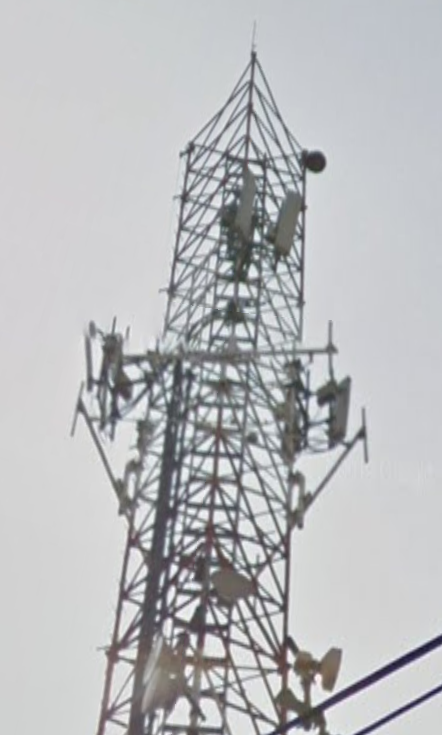
\includegraphics[width=0.3\textwidth]{imagenes/t11.png}
    \caption{Antena de la estación base.}
\end{figure}

\newpage
\subsection{Central Telmex Nezahualcóyotl}
\begin{itemize}
    \item \textbf{Dirección: }México, Estado de México, Nezahualcóyotl, Glorieta Bucareli, 
    Av. Adolfo López Mateos esquina, Evolución, 57700.
    \item \textbf{Coordenadas geográficas: }19.4092139 Norte, -99.024244 Oeste.
\end{itemize}

\subsection{Distancias}
\begin{itemize}
     \item \textbf{BS - MD: } 419 m.
     \item \textbf{BS - Central telefónica : } 1.38k m.
\end{itemize}

\subsection{Frecuencias de proveedor de servicios Telcel}
\textbf{Banda / Frecuencia para 3G}
\begin{itemize}
     \item B2 / 1900 MHz.
     \item B5 / 850 MHz.
\end{itemize}

\textbf{Banda / Frecuencia para 4G (LTE)}
\begin{itemize}
     \item B4 / 1700/2100 MHz.
\end{itemize}
    
\newpage
\section{Croquis del área de estudio}
\begin{figure}[ht]
    \centering
    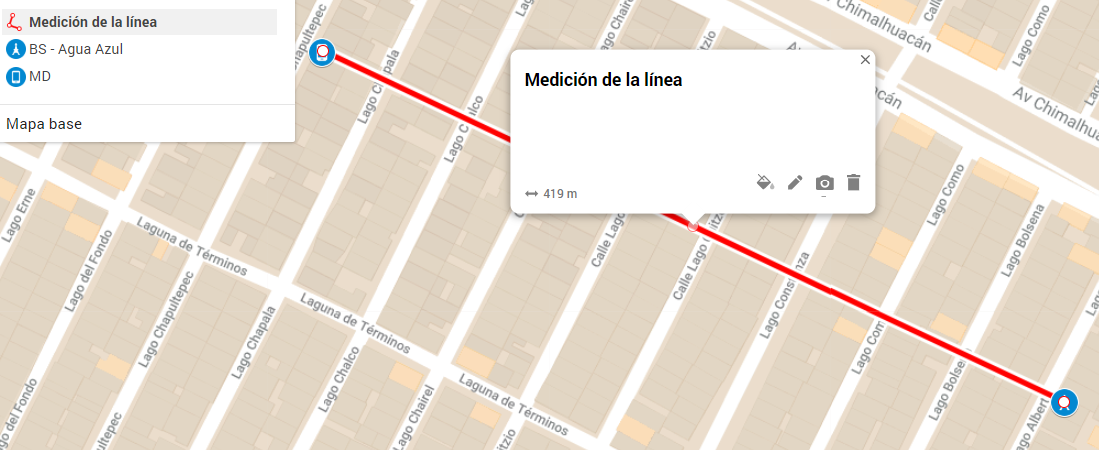
\includegraphics[width=.9\textwidth, angle=90]{imagenes/t13.png}
    \caption{Distancia MD - BS.}
\end{figure}

\newpage
\subsection{Perfil topográfico}
\begin{figure}[ht]
    \centering
    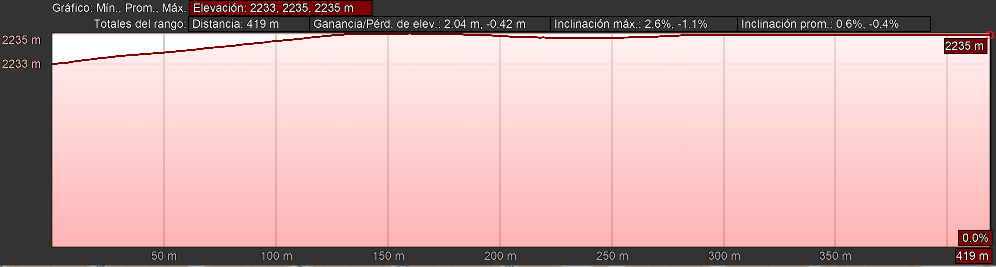
\includegraphics[width=.9\textwidth, angle=90]{imagenes/t14.png}
    \caption{Perfil topográfico.}
\end{figure}

\newpage
\section{Desarrollo}

\newpage
\section{Conclusión}

\end{document}